\documentclass[a4paper, 14pt]{extarticle}

\usepackage{../latexDependencies/misc/preamble2}

\geometry{a4paper}

% Название дисциплины
\newcommand{\subject}{Теория автоматов и алгоритмические языки} 

% Тип работы
% lab - для лабораторной работы 
% hw  - для домашней     работы
\newcommand{\task}{hw} 

% Номер работы
\newcommand{\taskNumber}{2-2} 

% % Название работы
% \newcommand{\taskNameOne}{Определение списка полиномов интерполяционного} 
% \newcommand{\taskNameTwo}{сплайна третьей степени единичного дефекта} 
% \newcommand{\taskNameThree}{для заданной сеточной функции} 

% Имя студента
\newcommand{\studentName}{Очкин Н.В.}

% Имя преподававателя
\newcommand{\teacherName}{Кутыркин В.А.}

% Группа
\newcommand{\group}{ФН11-52Б}

% Вариант
\newcommand{\variant}{9}

\let\emptyset\varnothing

\begin{document}

\graphicspath{ {../latexDependencies/images} } 
\normalsize

\newcommand{\printTask}{%
    \ifthenelse{\equal{\task}{lab}}{%
        лабораторной%
    }{%
        \ifthenelse{\equal{\task}{hw}}{%
            домашней%
        }{%
            Неизвестный тип задания%
        }%
    }%
}

\begin{titlepage}

    \begin{center}
        {\footnotesize \itshape Федеральное государственное бюджетное 
                       образовательное учреждение высшего образования}
    \end{center}

    \begin{minipage}[c]{0.1\textwidth}
        
\includegraphics[width=1.1\textwidth]{iconBMSTU}
    \end{minipage}
    \hfill
    \begin{minipage}[c]{0.9\textwidth}
        \centering
        \itshape
        \bfseries
        \small
        \guillemotleft Московский государственный технический университет \\
        имени Н.Э. Баумана\guillemotright \\
        (национальный исследовательский университет) \\
        (МГТУ им. Н.Э. Баумана) 
    \end{minipage}

    \vspace{0.5cm}
    \noindent\rule{\textwidth}{2pt} \\

    \noindent\uline{\textbf{ФАКУЛЬТЕТ} ФУНДАМЕНТАЛЬНЫЕ НАУКИ} \\
    \vspace{-5pt} \\
    \noindent\uline{\textbf{КАФЕДРА} ВЫЧИСЛИТЕЛЬНАЯ МАТЕМАТИКА И МАТЕМАТИЧЕСКАЯ} \\
    \vspace{-5pt} \\
    \noindent\uline{ФИЗИКА (ФН11)} \\
    \vspace{-5pt} \\
    \noindent\uline{\textbf{НАПРАВЛЕНИЕ ПОДГОТОВКИ} МАТЕМАТИКА И КОМПЬЮТЕРНЫЕ} \\
    \vspace{-5pt} \\
    \noindent\uline{НАУКИ (02.03.01)} \\

    \begin{center}
        \bfseries
        \textsc{О т ч е т} \\[10pt]
        по \printTask {} работе \textnumero {} \taskNumber
    \end{center}

    \vspace{10pt}

    \begin{center}
        \bfseries
        Вариант \textnumero {} \variant
    \end{center}

    \vspace{50pt}

    \hspace{10pt} 
    \noindent \textbf{Дисциплина:} \par
    \vspace{5pt}
    \hspace{10pt} 
    \noindent \subject

    \vspace{10pt}

    \begin{flushright}
        \renewcommand{\arraystretch}{3}
        \begin{tabular}{r r r}
            \multicolumn{1}{l}{Студент группы \uline{\group}} & 
            $\quad \underset{\text{(Подпись, дата)}}{\underline{\hspace{3cm}}} \quad$ & 
            \multicolumn{1}{c}{$\underset{\text{(И.О. Фамилия)}}{\uline{\textbf{\studentName}}}$} \\

            \multicolumn{1}{l}{Преподаватель} & 
            $\quad \underset{\text{(Подпись, дата)}}{\underline{\hspace{3cm}}} \quad$ & 
            \multicolumn{1}{c}{$\underset{\text{(И.О. Фамилия)}}{\uline{\textbf{\teacherName}}}$} \\
        \end{tabular}
    \end{flushright}

    \vfill

    \begin{center}
        \small
        Москва, 2024
    \end{center}
\end{titlepage}

\newgeometry{left=25mm, right=25mm, top=20mm, bottom=20mm}

\graphicspath{ {../latexDependencies/images/HW2-1} }

% Customize section, subsection, subsubsection and paragraph styles
\titleformat{\section}
  {\normalfont\large\bfseries}{\thesection}{2em}{}

\titleformat{\subsection}
  {\normalfont\normalsize\bfseries}{\thesubsection}{2em}{}

\titleformat{\subsubsection}
  {\normalfont\small\bfseries}{\thesubsubsection}{2em}{}

\titleformat{\paragraph}
  {\small\small\bfseries}{\theparagraph}{2em}{}

% \thispagestyle{empty}

% \null\newpage

% \setcounter{tocdepth}{5}
% \setcounter{secnumdepth}{5}

% \pagenumbering{roman}

% \tableofcontents
% \newpage

% \pagenumbering{arabic}
% \setcounter{page}{1}

\setstretch{1}
\linespread{1.1}

\setlength{\parindent}{0pt}

\fontsize{12pt}{16pt}\selectfont

\definecolor{myblue}{HTML}{0A88C2}
\definecolor{myred}{HTML}{FF1B1C}
\definecolor{mygreen}{HTML}{386641}

\lstdefinestyle{mystyle}{
    % frame=leftline, 
    % framesep=10pt, 
}

\lstset{style=mystyle, extendedchars=\true}

% --------------------------------------START--------------------------------------

\section*{Задача 1}

\subsection*{Задание}\vspace{-20pt}\rule{\linewidth}{0.1mm}

Написать простую программу на паскалеобразном языке с операторами 
\textbf{read} и \textbf{write}. С помощью (лексического анализатора) транслировать 
эту программу в языко токенов.

\subsection*{Решение}\vspace{-20pt}\rule{\linewidth}{0.1mm}

Запишем программу на языке программирования Pascal, принимающую на вход число и 
возвращующую true в случае если число четно, false если нечетно:\\

\vspace{50pt}

% \vfill

\vspace{-10pt}\rule{\linewidth}{0.1mm}

\begin{adjustbox}{center}
    \begin{adjustbox}{width=0.4\textwidth}
        \begin{lstlisting}[language=Pascal]
program isEven;

var
number: Integer;

begin
readln(number);

if (number mod 2 = 0) then
    writeln(true)
else
    writeln(false);
end.
        \end{lstlisting}
    \end{adjustbox}
\end{adjustbox}

\vspace{10pt}\rule{\linewidth}{0.1mm}

\newpage

\begin{table}[h!]
    \centering
    \resizebox{0.85\textwidth}{!}{ % Scale the table to the width of the text
    \setlength{\tabcolsep}{10pt} % Add horizontal space between columns
    \begin{tabular}{c c c c c}
    \toprule
     & 1 & 2 & 3 & 4 \\
    \midrule
     & Служебные & Идентификаторы & Константы & Разделители \\
     & слова     &                &           &             \\
    \midrule
    1 & program & isEven & 2 & ; \\[0.5em]
    2 & var & number & 0 & : \\[0.5em]
    3 & begin & & & ( \\[0.5em]
    4 & readln & & & ) \\[0.5em]
    5 & if & & & = \\[0.5em]
    6 & then & & & . \\[0.5em]
    7 & writeln & & & \\[0.5em]
    8 & else & & & \\[0.5em]
    9 & end & & & \\[0.5em]
    10 & mod & & & \\[0.5em]
    11 & true & & & \\[0.5em]
    12 & false & & & \\[0.5em]
    13 & Integer & & &
    \end{tabular}
    }
\end{table}

% \newpage

Сформируем список токенов:

\begin{center}
    (1, 1) \quad (2, 1) \quad (4, 1) \quad (1, 2) \quad (2, 2) \quad (4, 2) 
    \quad (1, 13) \quad (4, 1) \quad (1, 3) \\[1em]
    
    (1, 4) \quad (4, 3) \quad (2, 2) \quad (4, 4) \quad (4, 1) \quad (1, 5) 
    \quad (4, 3) \quad (2, 2) \quad (1, 10) \\[1em]
    
    (3, 1) \quad (4, 5) \quad (3, 2) \quad (4, 4) \quad (1, 6) \quad (1, 7) 
    \quad (4, 3) \quad (1, 11) \quad (4, 4) \\[1em]
    
    (1, 8) \quad (1, 7) \quad (4, 3) \quad (1, 12) \quad (4, 4) \quad (4, 1) 
    \quad (1, 9) \quad (4, 6) \quad \hphantom{(4, 6)}
\end{center}

\section*{Задача 2}

\subsection*{Задание}\vspace{-20pt}\rule{\linewidth}{0.1mm}

Провести синтаксический анализ арифметических выражений, переведя его
после этого в язык ПОЛИЗ. Реализовать вычисления, используя запись в
языке ПОЛИЗ, присвоив переменным фиксированные целые значения.

\subsection*{Исходные данные}\vspace{-20pt}\rule{\linewidth}{0.1mm}

\begin{equation*}
       -(-b) * (-2) + 2 - \sqrt{b^2 * 4} + 3 * 4
\end{equation*}

\subsection*{Решение}\vspace{-20pt}\rule{\linewidth}{0.1mm}

\vspace{10pt}

Запишем алфавит терминалов $T$ и алфавит нетерминалов $R$

\vspace{-5pt}

\begin{gather*}
    T = \left< \qquad + \qquad \oplus \qquad - \qquad \ominus \qquad * \qquad / \qquad \uparrow 
    \qquad \sqrt{} \qquad \left( \qquad \right)\qquad \right> \\[1em]
    R = \left< \qquad \text{C} \qquad \text{Y} \qquad \text{M} \qquad \text{S} \qquad \right> \\[1em]
    B: \begin{cases}
        1) \quad \text{S} \rightarrow \hspace{3pt} \stackrel{\text{а}}{\text{MYC}} \quad | \quad \oplus \stackrel{\text{б}}{\text{MYC}} \quad | \quad \ominus \stackrel{\text{в}}{\text{MYC}} \\[0.5em]
        2) \quad \text{C} \rightarrow \hspace{3pt} \stackrel{\text{а}}{\varepsilon} \quad | \quad + \stackrel{\text{б}}{\text{MYC}} \quad | \quad - \stackrel{\text{в}}{\text{MYC}} \\[0.5em] 
        3) \quad \text{Y} \rightarrow \hspace{3pt} \stackrel{\text{а}}{\varepsilon} \quad | \quad * \stackrel{\text{б}}{\text{MY}} \quad | \quad / \stackrel{\text{в}}{\text{MY}} \quad | \quad \uparrow \stackrel{\text{г}}{\text{MY}} \\[0.5em]
        4) \quad \text{M} \rightarrow \hspace{3pt} \stackrel{\text{а}}{x} \quad | \quad \stackrel{\text{б}}{\text{(S)}} \quad | \quad \stackrel{\text{в}}{\sqrt{\hphantom{1}}(S)} \\[0.5em]
    \end{cases}
\end{gather*}

Редуцируем заданное арифметическое выражение до арифметического выражения с 
одной переменной x:

\begin{equation*}
    - \hspace{3pt} ( \hspace{3pt} - \hspace{3pt} x \hspace{3pt} ) \hspace{3pt} * \hspace{3pt} ( \hspace{3pt} - \hspace{3pt} x \hspace{3pt} ) \hspace{3pt} + \hspace{3pt} x \hspace{3pt} - \hspace{3pt} \sqrt{\hphantom{1}} \hspace{3pt} ( \hspace{3pt} x \hspace{3pt} \uparrow \hspace{3pt} x \hspace{3pt} * \hspace{3pt} x \hspace{3pt} ) \hspace{3pt} + \hspace{3pt} x \hspace{3pt} * \hspace{3pt} x
\end{equation*}

Проведем синтаксический анализ

\begin{figure}[h]
    \centering
    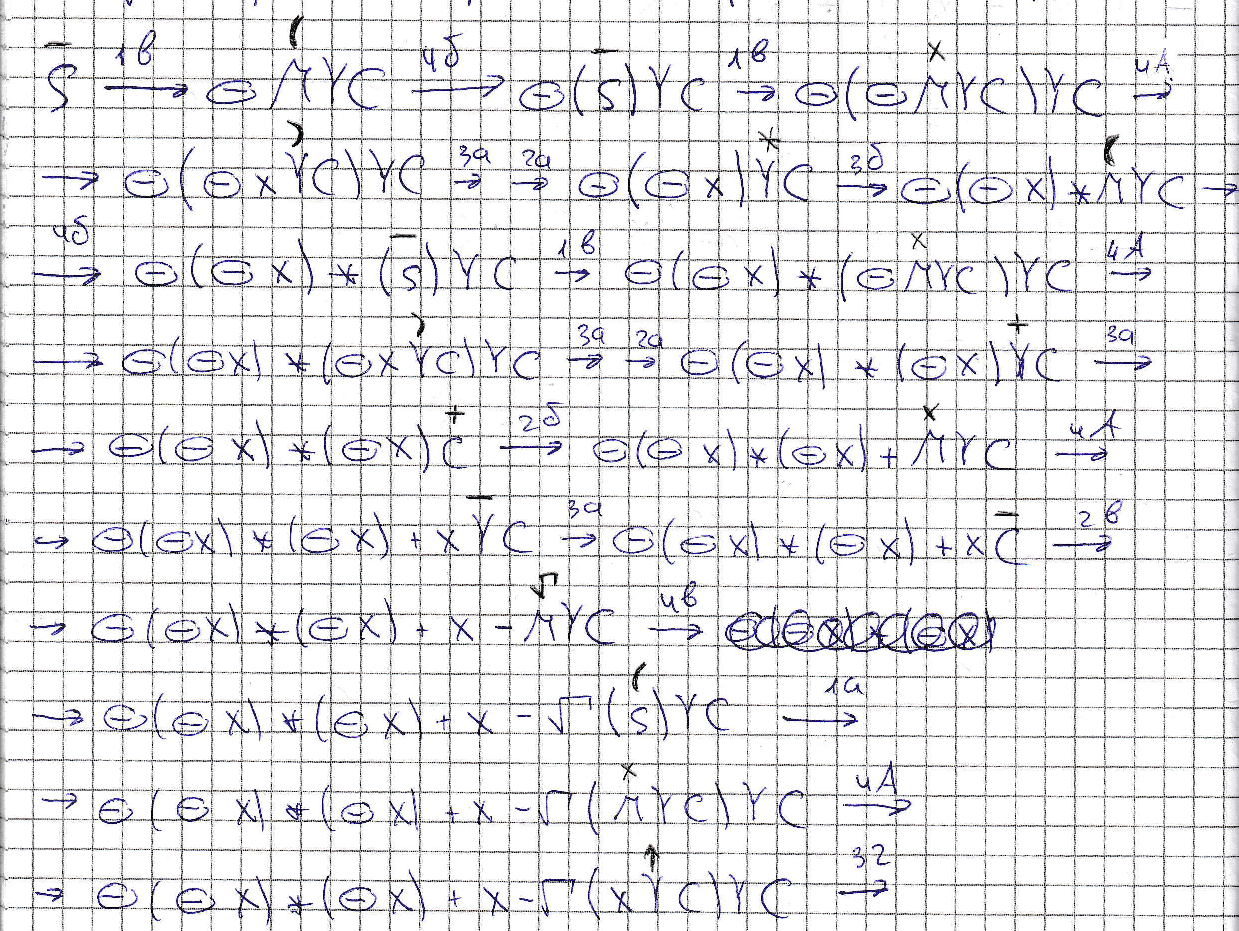
\includegraphics[width=\textwidth,height=\textheight,keepaspectratio]{graphics/1-cropped}
\end{figure}

\begin{figure}[h]
    \centering
    \rotatebox{180}{
        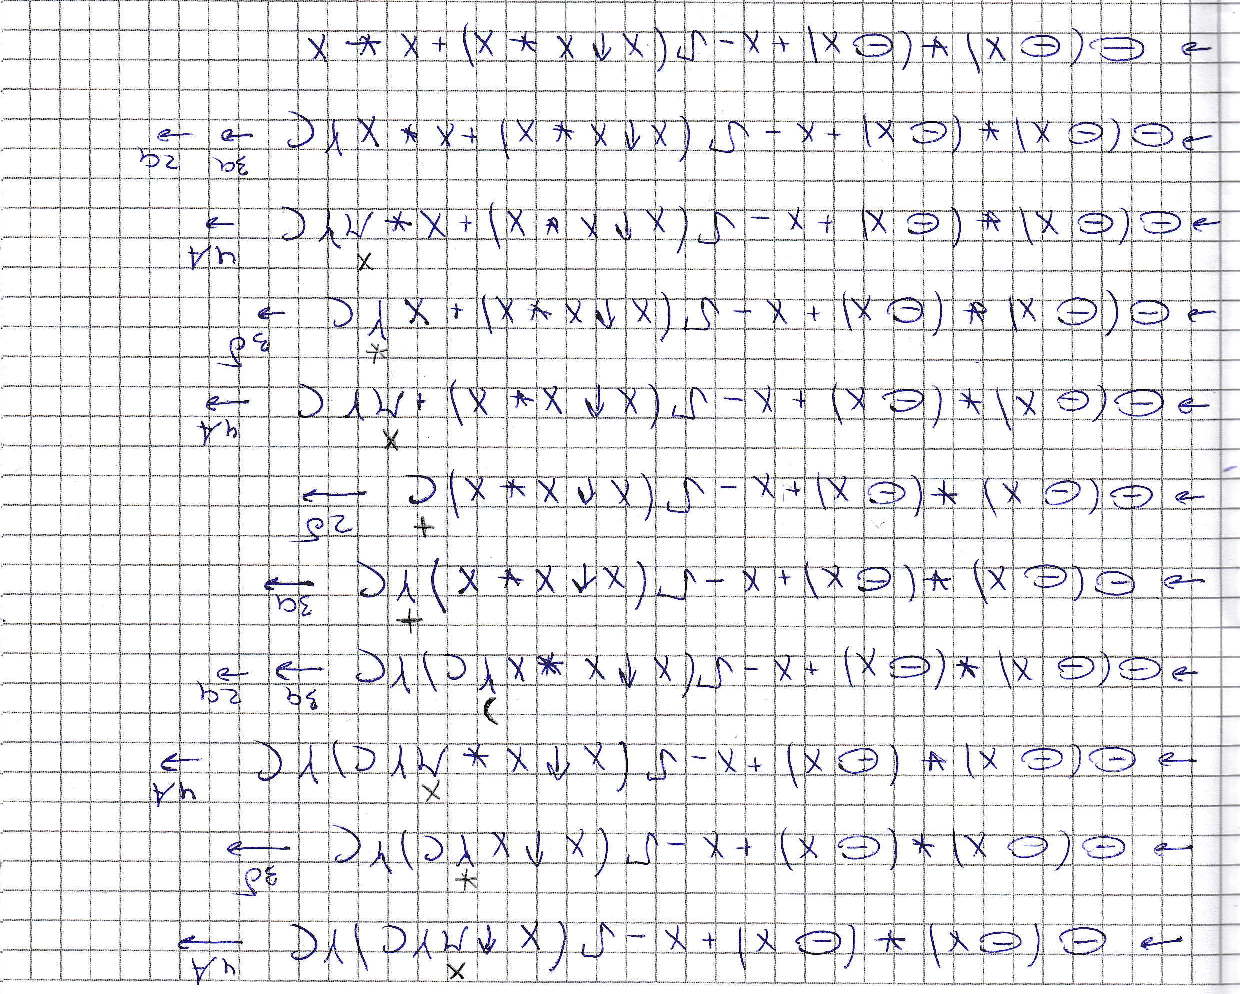
\includegraphics[width=\textwidth,height=\textheight,keepaspectratio]{graphics/2-cropped}
    }
\end{figure}

Итого получим

\begin{equation*}
    \ominus \hspace{3pt} ( \hspace{3pt} \ominus \hspace{3pt} x \hspace{3pt} ) \hspace{3pt} * \hspace{3pt} ( \hspace{3pt} \ominus \hspace{3pt} x \hspace{3pt} ) \hspace{3pt} + \hspace{3pt} x \hspace{3pt} - \hspace{3pt} \sqrt{\hphantom{1}} \hspace{3pt} ( \hspace{3pt} x \hspace{3pt} \uparrow \hspace{3pt} x \hspace{3pt} * \hspace{3pt} x \hspace{3pt} ) \hspace{3pt} + \hspace{3pt} x \hspace{3pt} * \hspace{3pt} x
\end{equation*}

Синтаксический анализ был проведе корректно, было получено исходное выражение.\\
Рассмотрим арифметическое выражение:
\begin{equation}
    \rotatebox{90}{\(\triangle\)} \hspace{3pt} \ominus \hspace{3pt} ( \hspace{3pt} \ominus \hspace{3pt} b \hspace{3pt} ) \hspace{3pt} * \hspace{3pt} ( \hspace{3pt} \ominus \hspace{3pt} 2 \hspace{3pt} ) \hspace{3pt} + \hspace{3pt} 2 \hspace{3pt} - \hspace{3pt} \sqrt{\hphantom{1}} \hspace{3pt} ( \hspace{3pt} 2 \hspace{3pt} \uparrow \hspace{3pt} 4 \hspace{3pt} * \hspace{3pt} 3 \hspace{3pt} ) \hspace{3pt} + \hspace{3pt} 4 \hspace{3pt} * \hspace{3pt} x \hspace{3pt} \reflectbox{\rotatebox{90}{\(\triangle\)}}
\end{equation}

Запишем в виде ниже прилагаемой таблицы протокол генерации компиляции этого
выражения в слово языка ПОЛИЗ. Предполагается, что в начале генерации символ $\rotatebox{90}{\(\triangle\)}$
находится на дне стека.

\newpage

\begin{figure}[H]
    \centering
    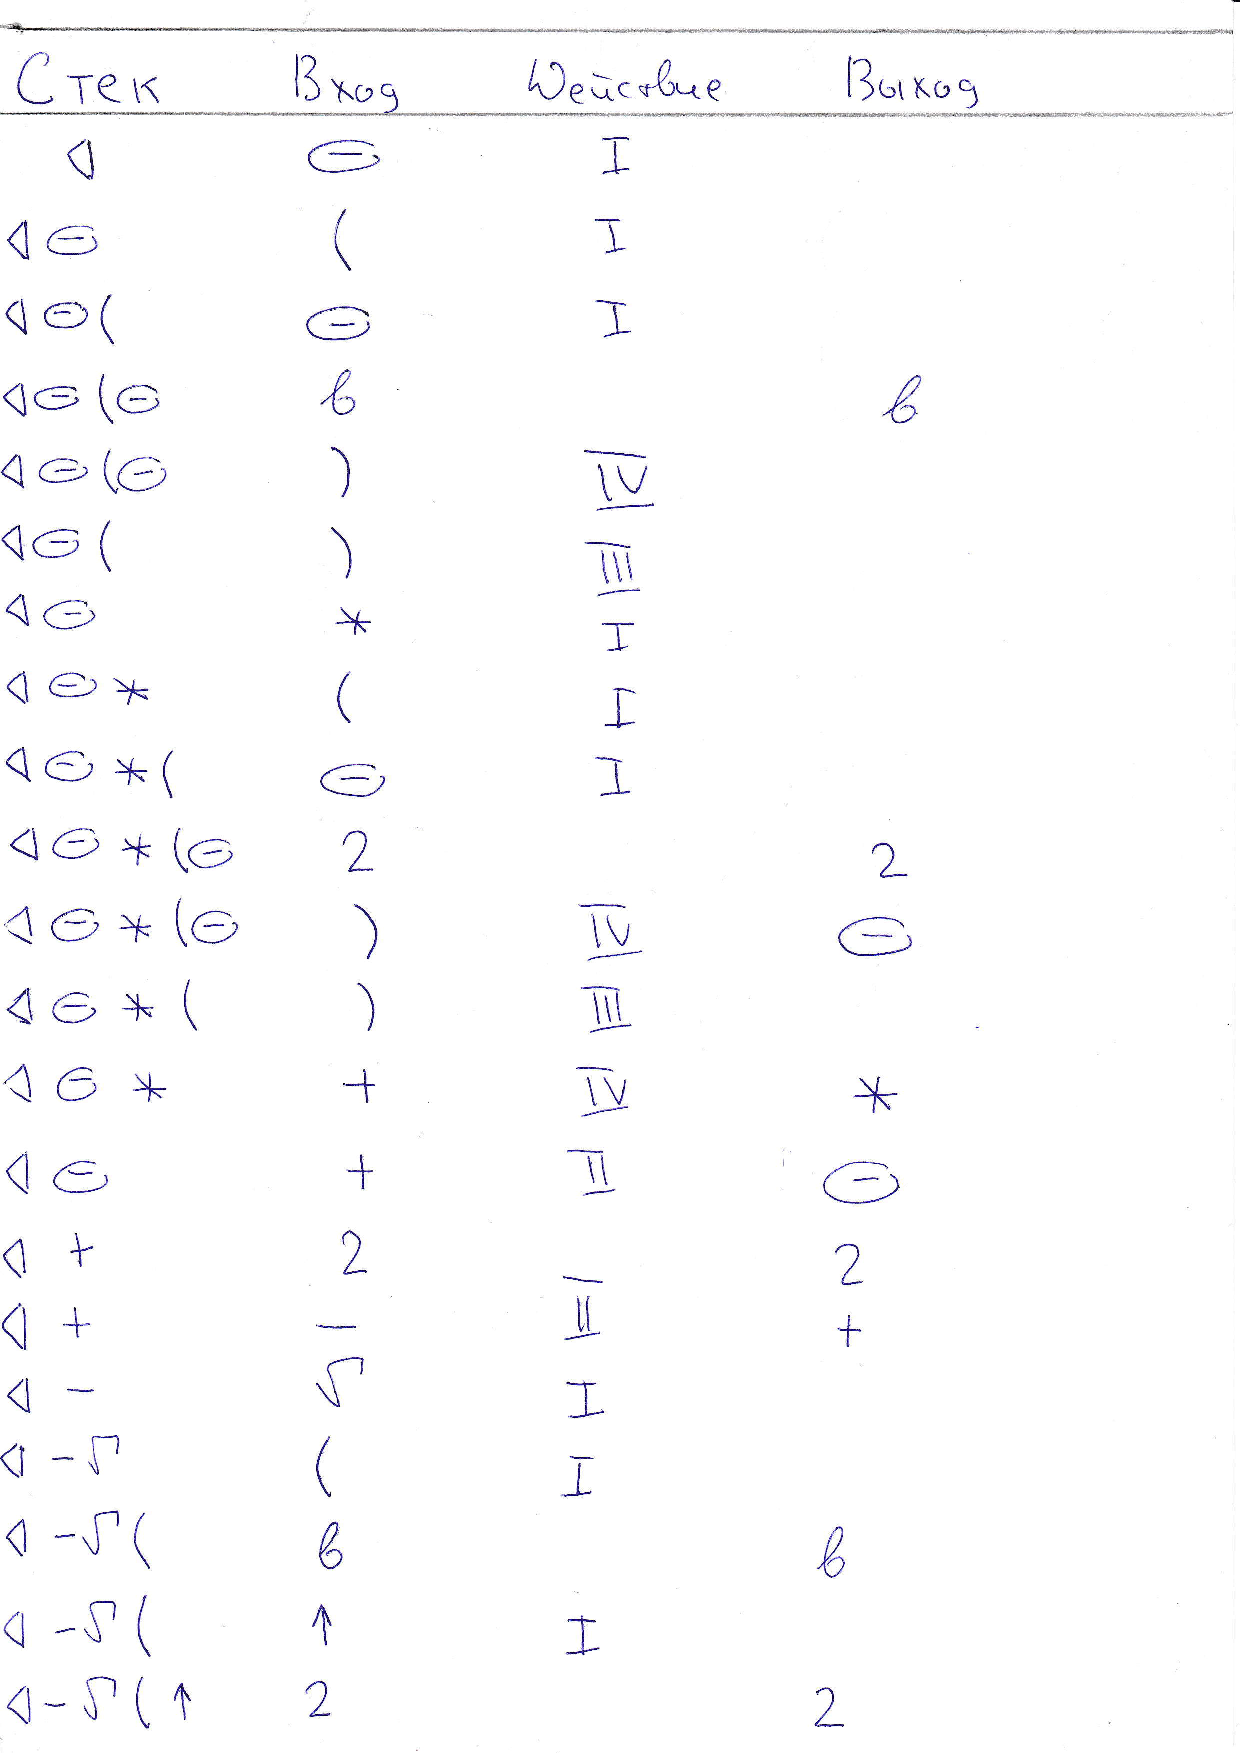
\includegraphics[width=\textwidth,height=\textheight,keepaspectratio]{graphics/3}
\end{figure}

\newpage

\begin{figure}[H]
    \centering
    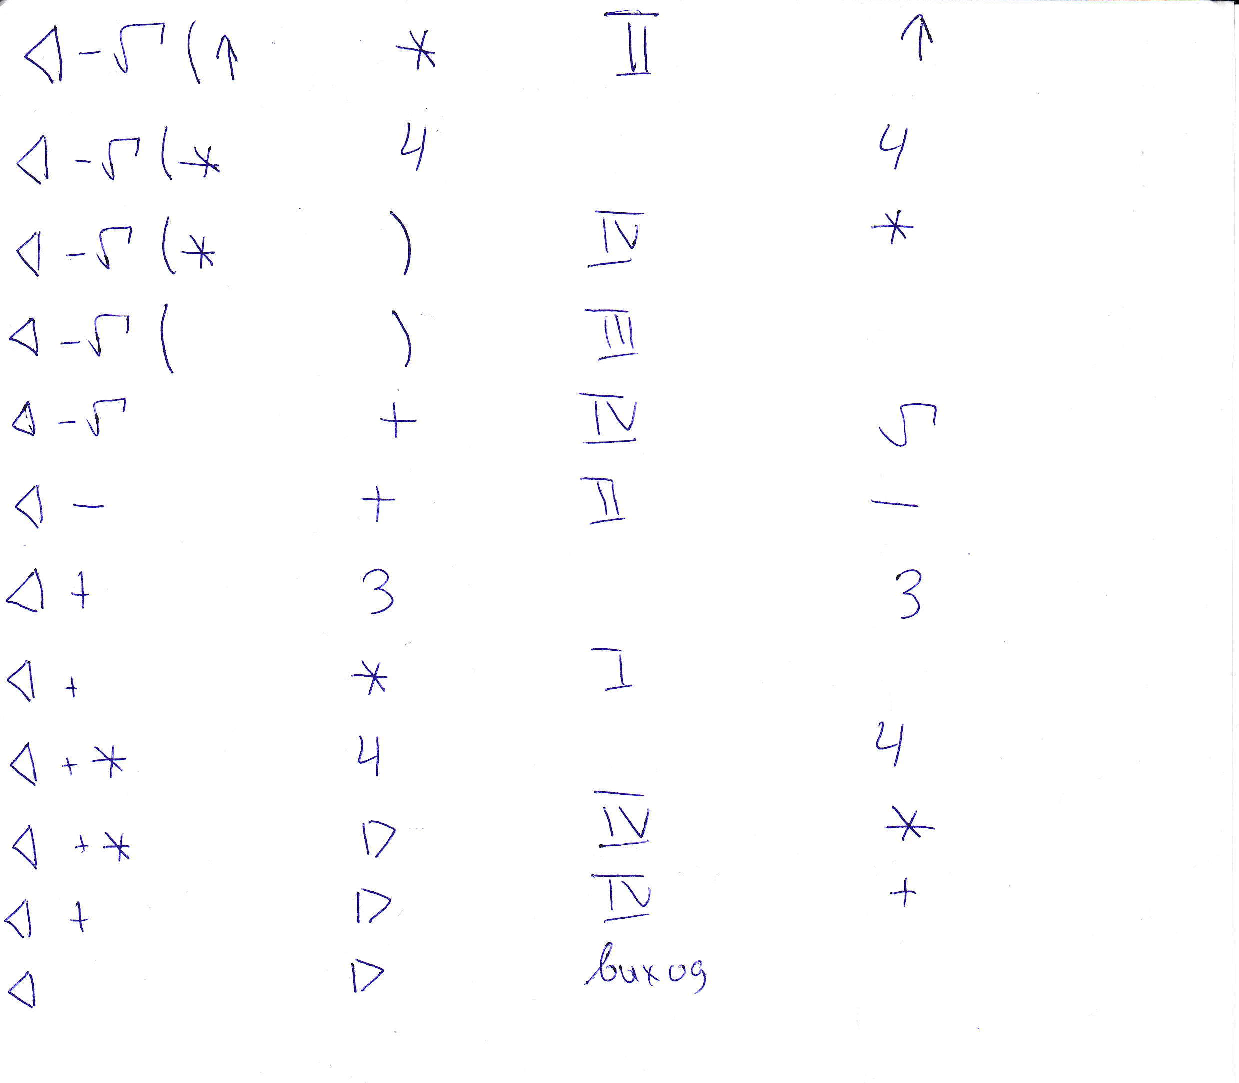
\includegraphics[width=\textwidth,height=\textheight,keepaspectratio]{graphics/4-cropped}
\end{figure}

Итого получили слово на языке ПОЛИЗ:

\begin{equation}
    b \hspace{3pt} \ominus \hspace{3pt} \left< 2 \right> \hspace{3pt} \ominus \hspace{3pt} * \hspace{3pt} \ominus \hspace{3pt} \left< 2 \right> \hspace{3pt} + \hspace{3pt} b \hspace{3pt} \left< 2 \right> \hspace{3pt} \uparrow \hspace{3pt} \left< 4 \right> \hspace{3pt} * \hspace{3pt} \sqrt{\hphantom{1}} \hspace{3pt} - \hspace{3pt} \left< 3 \right> \hspace{3pt} \left< 4 \right> \hspace{3pt} * \hspace{3pt} + 
\end{equation}

Для вычислений положим, что $b = \left< 1 \right>$. Тогда, проивзедя вычисления в 
арифметическом выражении (1), получим:

\begin{gather*}
    \ominus(\ominus \left< 1 \right>) * (\ominus \left< 2 \right>) + \left< 2 \right> - 
    \sqrt{\hphantom{1}} (\left< 1 \right> \uparrow \left< 2 \right> * \left< 4 \right>) + 
    \left< 3 \right> * \left< 4 \right> = \\[0.5em]
    = \ominus (- \left< 1 \right> * (- \left< 2 \right>)) + \left< 2 \right> - \sqrt{\left< 4 \right>} + 
    \left< 12 \right> = \\[0.5em]
    = - \left< 2 \right> + \left< 2 \right> - \left< 2 \right> + \left< 12 \right> =\\[0.5em]
\end{gather*}

\vspace{-50pt}

\begin{equation}
    = \left< 10 \right>
\end{equation}

Теперь с помощью стека проведем вычисление выражения (1), используя его представление (2) в языке 
ПОЛИЗ:

\newpage

\begin{table}[h!]
    \centering
    \renewcommand{\arraystretch}{1.5} % Increase vertical space between rows
    \resizebox{0.95\textwidth}{!}{ % Scale the table to the width of the text
    \setlength{\tabcolsep}{10pt} % Add horizontal space between columns
    \begin{tabular}{c | c c c c c c c c c c c c}
    \hline
    Операция & $\ominus$ & $\ominus$ & * & $\ominus$ & + & $\uparrow$ & * & $\sqrt{\hphantom{1}}$ & - & * & + &  \\
    \hline
    \multirow{3}{*}{Стек} &    &      &      &   &    & 2 & 4 &   &   & 4  &    &    \\
                          &    & 2    & -2   &   & 2  & 1 & 1 & 4 & 2 & 3  & 12 &    \\
                          & 1  &  -1  & -1   & 2 & -2 & 0 & 0 & 0 & 0 & -2 & -2 & 10 \\
    \end{tabular}
    }
\end{table}

Получили тот же результат, что и в (3).

\vfill

\end{document}
